%%%%%%%%%%%%%%%%%%%%%%%%%%%%%%%%%%%%%%%%%
% Beamer Presentation
% LaTeX Template
% Version 1.0 (10/11/12)
%
% This template has been downloaded from:
% http://www.LaTeXTemplates.com
%
% License:
% CC BY-NC-SA 3.0 (http://creativecommons.org/licenses/by-nc-sa/3.0/)
%
%%%%%%%%%%%%%%%%%%%%%%%%%%%%%%%%%%%%%%%%%

%----------------------------------------------------------------------------------------
%	PACKAGES AND THEMES
%----------------------------------------------------------------------------------------
%!TEX encoding = UTF-8 Unicode

\documentclass{beamer}
\usepackage[utf8]{inputenc}
\usepackage{dsfont}
\usepackage{braket}
\usepackage{scalerel}
\usepackage{gensymb}
\usepackage{verbatim}
\usepackage{dsfont}
\usepackage[autostyle]{csquotes}
\usepackage{pgfpages}
\setbeamertemplate{note page}[plain]
%\setbeameroption{show notes on second screen=right}

\usepackage[
    backend=biber,
    style=authoryear-icomp,
    sortlocale=de_DE,
    natbib=true,
    url=false, 
    doi=true,
    eprint=false
]{biblatex}
\addbibresource{biblio.bib}


\mode<presentation> {

\usetheme{Warsaw}

}

\usepackage{graphicx} % Allows including images
\usepackage{booktabs} % Allows the use of \toprule, \midrule and \bottomrule in tables

%----------------------------------------------------------------------------------------
%	TITLE PAGE
%----------------------------------------------------------------------------------------


\title[The computational power of linear optics]{The computational power of linear optics} % The short title appears at the bottom of every slide, the full title is only on the title page

\author[Federico Belliardo]
{
Federico Belliardo\\
\vspace{10pt}
} 

\institute[Unipi] % Your institution as it will appear on the bottom of every slide, may be shorthand to save space
{
Università di Pisa\\ % Your institution for the title page
\medskip
}
\date{\today} % Date, can be changed to a custom date

\begin{document}

%------------------------------------------
\begin{frame}
\titlepage % Print the title page as the first slide
\end{frame}

%------------------------------------------
\begin{frame}
\begin{center}

\begin{block}{}
\begin{center}
What does it means linear optics?
\end{center}
\end{block}

\begin{itemize}
\item Input modes $\rightarrow a_k$\\
\item Output modes: $\rightarrow b_k$
\end{itemize}

\begin{figure}[!htb]
\centering
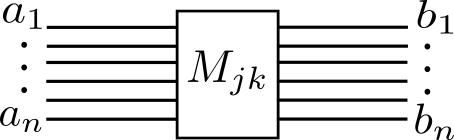
\includegraphics[scale=.4]{immagini/IO.png}
\end{figure}
\begin{equation*}
b_j^{\dagger} = \sum_{k} M_{jk} a_k^{\dagger} 
\end{equation*}

%Physical examples: Beam splitters, phase plates, polarizing beam splitters, mirrors.\\
%Non linear elements: Squeezers, detectors.

\end{center}
\end{frame}

%------------------------------------------
\begin{frame}
\begin{center}

\begin{itemize}
\item Phase shifter, $\ket{n} \rightarrow e^{i n \phi} \ket{n}$ 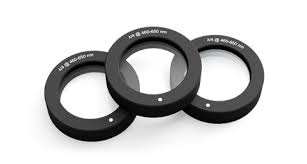
\includegraphics[height= 3 \baselineskip]{immagini/waveplates.jpeg}
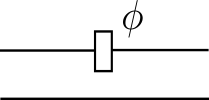
\includegraphics[height= 2 \baselineskip]{immagini/Rz.png}
\vspace{15pt}
\item Beamsplitters, 
$
\begin{pmatrix}
b_{1}^{\dagger}\\
b_{2}^{\dagger}
\end{pmatrix} = 
\begin{pmatrix}
\cos \theta & - e^{i \phi} \sin \theta \\
e^{-i \phi} \sin \theta & \cos \theta
\end{pmatrix}
\begin{pmatrix}
a_{1}^{\dagger}\\
a_{2}^{\dagger}
\end{pmatrix}
$
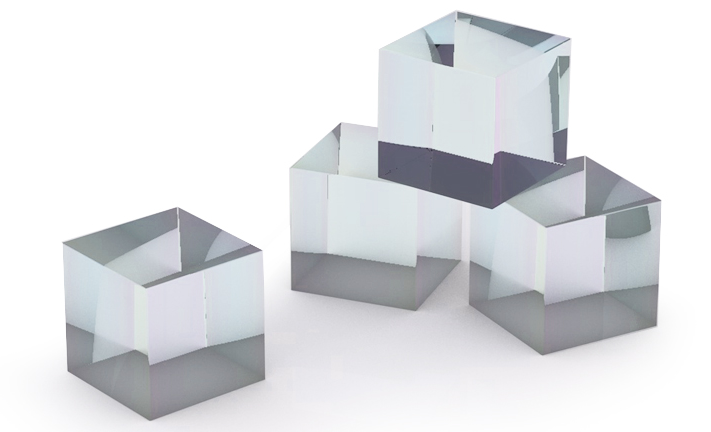
\includegraphics[height= 4 \baselineskip]{immagini/beamsplitter.png}
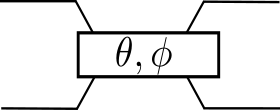
\includegraphics[height= 2 \baselineskip]{immagini/Ry.png}\\
\vspace{15pt}
\item Mirrors, Identity operators 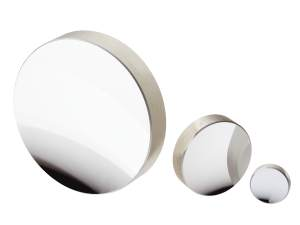
\includegraphics[height= 4 \baselineskip]{immagini/mirror.jpg}

\end{itemize}

\end{center}
\end{frame}

%------------------------------------------
\begin{frame}
\begin{center}
A generic unitary $U$ acting on the modes $a_i$ can be decomposed in a series of beamsplitters and phase shifter.

\begin{equation*}
U = BS_{N, N-1} \cdot BS_{N, N-2} \dots BS_{N-1, N-3} \cdot BS_{2, 1} \cdot D
\end{equation*}

\begin{figure}[!htb]
\centering
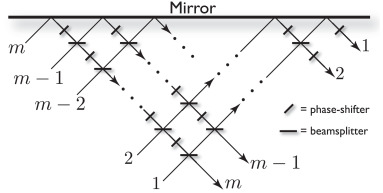
\includegraphics[scale=1]{immagini/decomposition2.jpg}
\end{figure}

$BM_{i, j}$ is a beamsplitter applied on modes $i, j$ and $D$ unitary diagonal matrix representing the application of a phase shifter on each mode. 

\end{center}
\end{frame}

%------------------------------------------
\begin{frame}
\begin{center}

This doesn't means we have implement universal quantum computing!
There is no qubit encoding in this scheme!

%, the unitary is only acting on the modes as a change of basis.

\end{center}
\end{frame}

%------------------------------------------
\begin{frame}{Qubit encodings}
\begin{center}

\begin{itemize}
\item Single rail: $\ket{\psi} = \alpha \ket{0} + \beta \ket{1}$ (Lund \& Ralph 2002). Difficult single qubit gates.

\item Polarization $\ket{\psi} = \alpha \ket{H} + \beta \ket{V}$.

\begin{figure}[!htb]
\centering
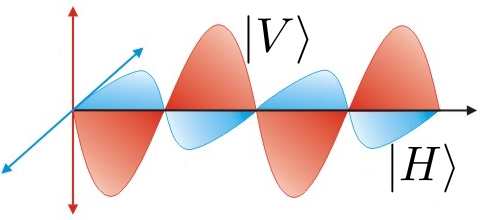
\includegraphics[scale=.3]{immagini/polarization.png}
\end{figure}


\item Dual rail encoding $\ket{\psi} = \alpha \ket{10} + \beta \ket{01}$.
\end{itemize}

\begin{figure}[!htb]
\centering
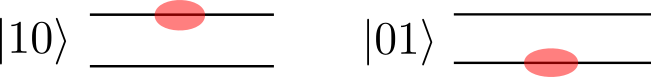
\includegraphics[scale=0.5]{immagini/dualRail.png}
\end{figure}

\end{center}
\end{frame}

%------------------------------------------
\begin{frame}
\begin{center}

Polarization and dual rail can be converted into one another:

\begin{figure}[!htb]
\centering
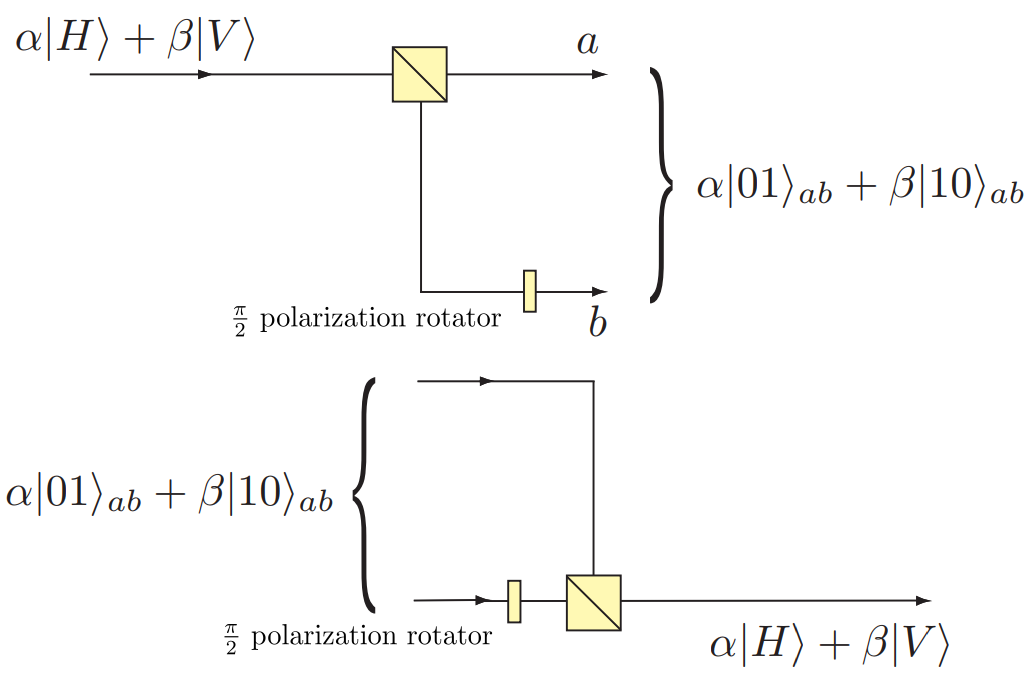
\includegraphics[scale=.25]{immagini/conversion2.png}
\end{figure}

\end{center}
\end{frame}

%------------------------------------------
\begin{frame}
\begin{center}

Coherent state encoding $\ket{\psi} = c_0 \ket{\alpha} + c_1 \ket{ \text{-} \alpha}$.\\
\textbf{Cons}:
\begin{itemize}
\item Difficult single qubit gates. 
\item Non orthogonal $\langle \alpha | \beta \rangle \sim e^{-|\alpha- \beta|^2}$.
\end{itemize}
\textbf{Pros}:
\begin{itemize}
\item Easy entanglement production (beamsplitters).
\end{itemize}

\begin{figure}[!htb]
\centering
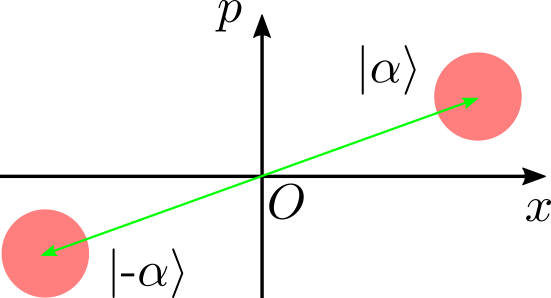
\includegraphics[scale=.4]{immagini/coherent.png}
\end{figure}

\end{center}
\end{frame}

%------------------------------------------
\begin{frame}
\begin{center}
\begin{block}{}
\begin{center}
How to create entanglement between photonic qubits?
\end{center}
\end{block}
\end{center}
\end{frame}


%------------------------------------------
\begin{frame}
\begin{center}
Cross-Kerr non linearities $H = - \hbar \chi a_i^{\dagger} a_i b_i^{\dagger} b_i$.\\
If a photon is in mode $c_i$ then $a_o = b_i$, $b_o = a_i$ (Fredkin gate, controlled SWAP).

\begin{figure}[!htb]
\centering
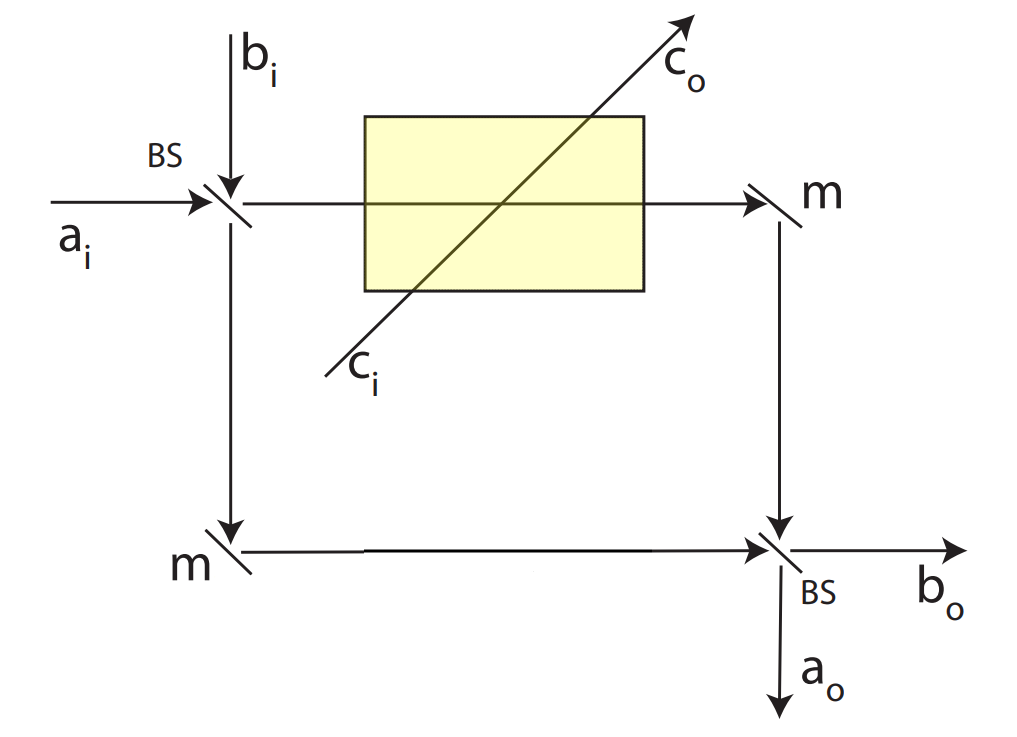
\includegraphics[scale=.17]{immagini/CrossKerr.png}
\end{figure}

CNOT with dual rail encoding. Strong non linearities are required.
\end{center}
\end{frame}

%------------------------------------------
\begin{comment}
\begin{frame}{Spin off - Quantum Non Demolition measurements}
\begin{center}
The Kerr effect can be used to perform quantum non demolition measurements.

\begin{figure}[!htb]
\centering
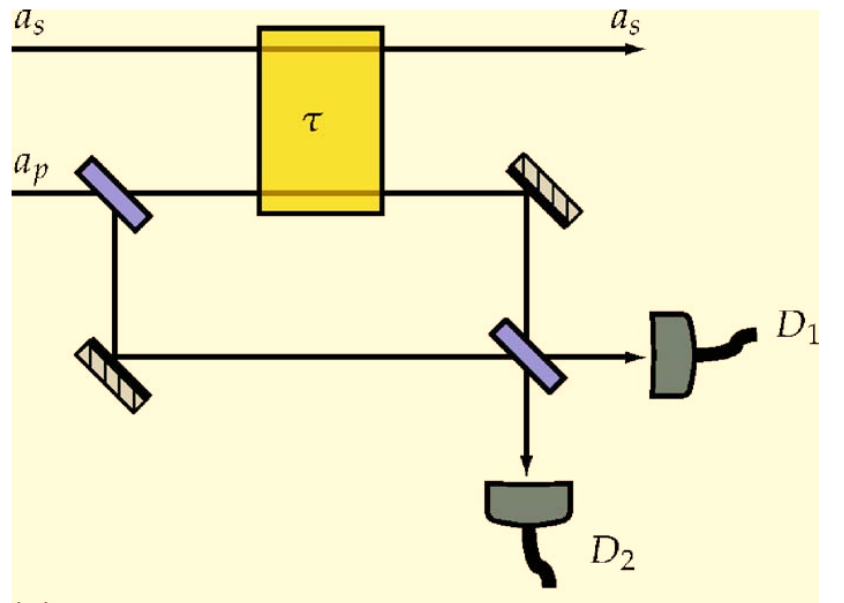
\includegraphics[scale=.30]{immagini/NDM.png}
\end{figure}

\end{center}
\end{frame}
\end{comment}

%------------------------------------------
\begin{frame}{The computational power of linear optics}
\begin{center}

Interactions through non linear elements comes with high absorption and decoherence.

\begin{block}{}
\begin{center}
What can we do with linear optics alone?
\end{center}
\end{block}
\vspace{20pt}
Surprisingly linear optic allows to implement the universal quantum computer \textbf{efficiently} (with polynomial overhead).\\
\vspace{20pt}
``Efficient Linear Optics Quantum Computation''\\
E. Knill, R. Laflamme, G. Milburn\\
2000

\end{center}
\end{frame}

%------------------------------------------
\begin{frame}
\begin{center}

It is fundamental to have feedforward measurement: results ($R$) of photodetectors in midway of computation determine successive operations.

\begin{figure}[!htb]
\centering
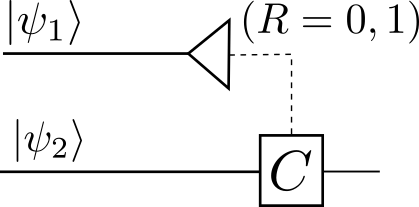
\includegraphics[scale=.5]{immagini/feedforward.png}
\end{figure}

\begin{block}{}
\begin{center}
Measurement non linearity is the only required for QC!
\end{center}
\end{block}

\end{center}
\end{frame}


%------------------------------------------
\begin{frame}
\begin{center}

Single qubit gates can be easily implemented with beam splitters and a phase shifter:

\begin{figure}[!htb]
\centering
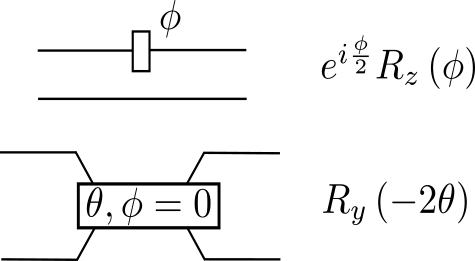
\includegraphics[scale=.5]{immagini/single.png}
\end{figure}

Euler decomposition: $U = e^{i \alpha} R_{z} \left( \beta \right) R_{y} \left( \gamma \right) R_{z} \left( \delta \right)$.

\begin{figure}[!htb]
\centering
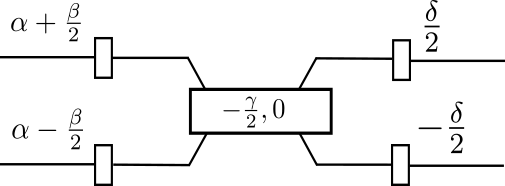
\includegraphics[scale=.5]{immagini/U.png}
\end{figure}

\end{center}
\end{frame}

%------------------------------------------
\begin{frame}
\begin{center}
In order to do universal quantum computation we must be able to implement a CNOT (CX). Equivalently we implement a CSIGN (CZ):

\begin{figure}[!htb]
\centering
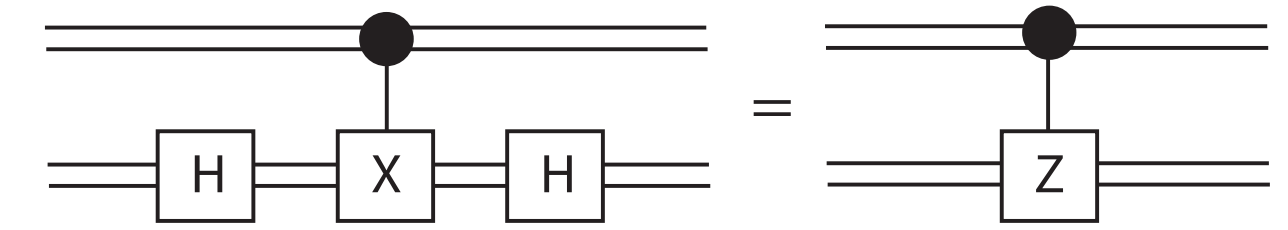
\includegraphics[scale=.25]{immagini/cnotcsign.png}
\end{figure}

\begin{block}{}
\begin{center}
We will realize CZ through an \textbf{auxiliary} NS gate.
\end{center}
\end{block}{}

\end{center}
\end{frame}

%------------------------------------------
\begin{frame}{Non linear sign shift (NS)}
\begin{center}
\begin{equation*}
\alpha \ket{0} + \beta \ket{1} + \gamma \ket{2} \rightarrow \alpha \ket{0} + \beta \ket{1} - \gamma \ket{2}
\end{equation*}

\begin{figure}[!htb]
\centering
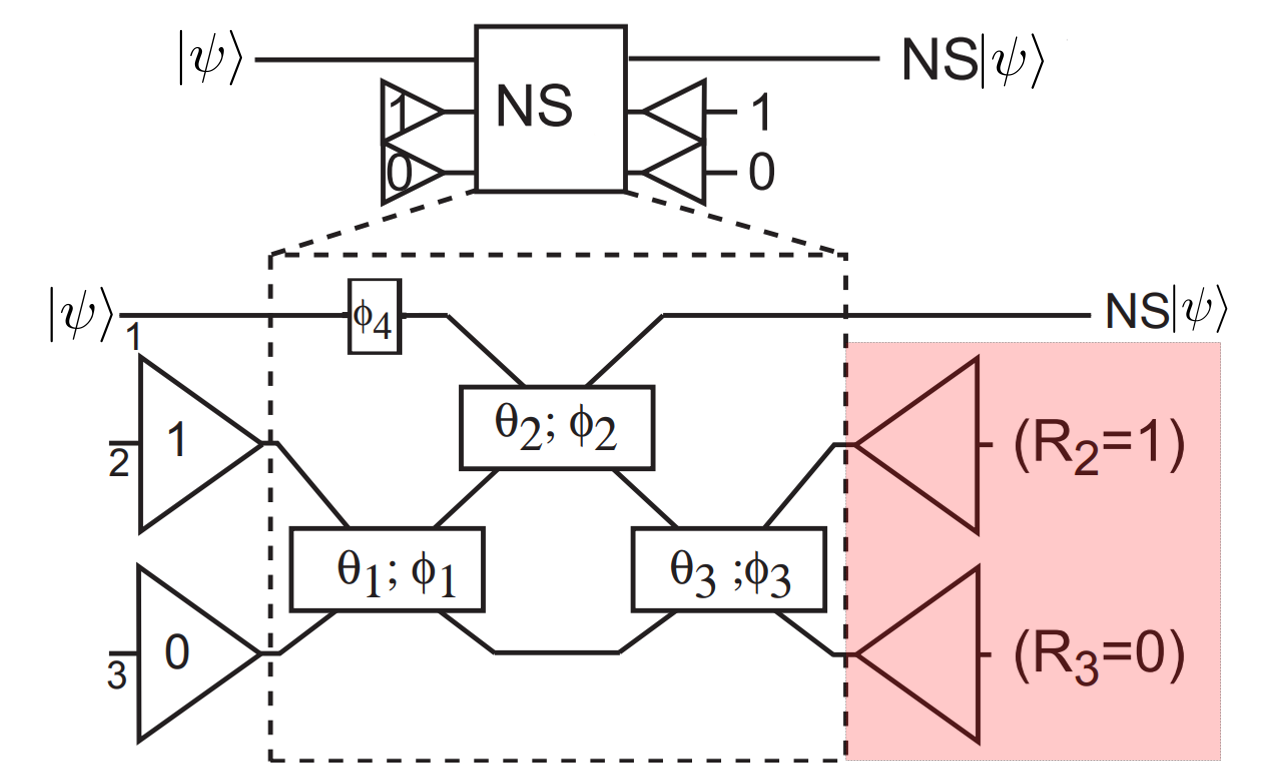
\includegraphics[scale=.20]{immagini/ns.png}
\end{figure}

The two ancillary qubits must be measured in $R_2 = 1$ and $R_3 = 0$.

\end{center}
\end{frame}

%------------------------------------------
\begin{frame}
\begin{center}

NS is a non deterministic heralded quantum gate.\\
\vspace{20pt}
The success probability of applying NS is $p = \frac{1}{4}$, but we know when it fails.

\end{center}
\end{frame}

%------------------------------------------
\begin{frame}
\begin{center}

We build CSIGN via a double application of NS:

\begin{figure}[!htb]
\centering
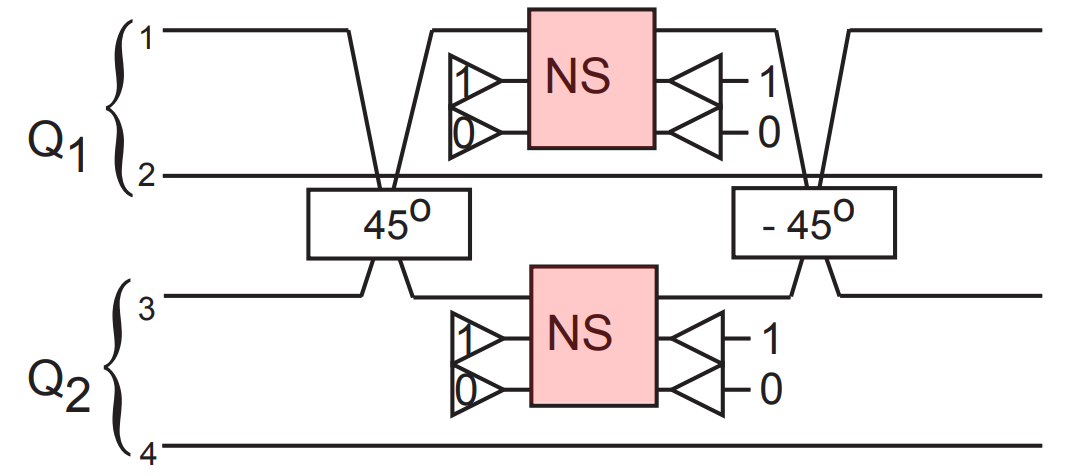
\includegraphics[scale=.25]{immagini/csign.png}
\end{figure}
\begin{equation*}
p = \frac{1}{4} \times \frac{1}{4} = \frac{1}{16}
\end{equation*}
If the gate fail the quantum information is \textbf{lost}!.\\
Notice that only modes $1$ and $3$ interact.

\end{center}
\end{frame}

%------------------------------------------
\begin{frame}{Teleportation trick}
\begin{center}

After the application of $N$ gates the probability of success is $p^{N}  \rightarrow 0$ \scalerel*{
\includegraphics{immagini/smile.png}}{B}\\

\begin{block}{}
\begin{center}
Can we make a deterministic gate? Or at least enhance the probability $p$ of performing the computation?
\end{center}
\end{block}

\vspace{10pt}

\textbf{Gate teleportation} by Gottesman \& Chuang (1999).

\end{center}
\end{frame}

%-------------------------------------------
\begin{frame}
\begin{center}

\begin{block}{}
\begin{center}
Qubit teleportation protocol:
\end{center}
\end{block}

\begin{figure}[!htb]
\centering
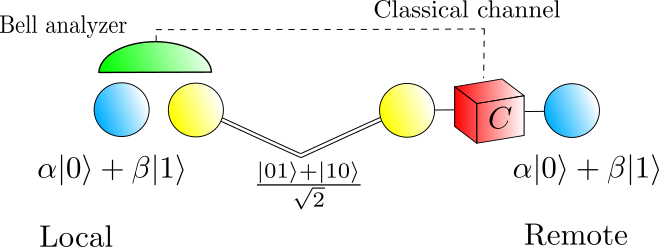
\includegraphics[scale=.60]{immagini/teleCartoon.png}
\end{figure}

\end{center}
\end{frame}

%------------------------------------------
\begin{frame}
\begin{center}

Qubit teleportation in optical modes.

\begin{figure}[!htb]
\centering
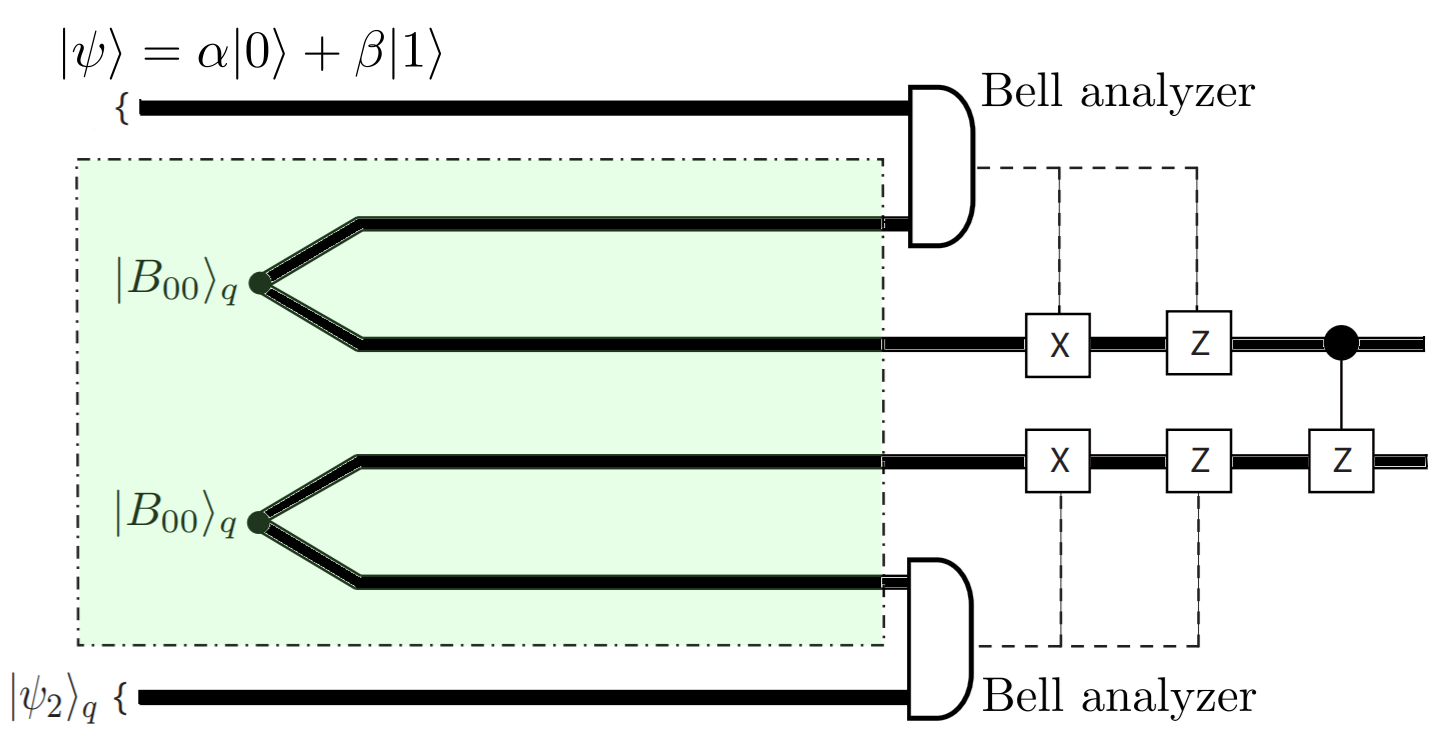
\includegraphics[scale=.20]{immagini/tele.png}
\end{figure}

\end{center}
\end{frame}

%------------------------------------------
\begin{frame}
\begin{center}

We shift the entangling gate into the preparation step (green stage) by commuting CSIGN with the classically controlled gates $X$ and $Y$.\\

\begin{align*}
& \text{CSIGN} \left( \sigma_x \otimes \mathds{1} \right) \text{CSIGN} =\sigma_x \otimes \sigma_z \\
& \text{CSIGN} \left( \mathds{1} \otimes \sigma_x \right) \text{CSIGN} = \sigma_z \otimes \sigma_x \\
& \text{CSIGN} \left( \sigma_z \otimes \mathds{1} \right) \text{CSIGN} = \sigma_z \otimes \mathds{1} \\
& \text{CSIGN} \left( \mathds{1} \otimes \sigma_x \right) \text{CSIGN} = \sigma_z \otimes \sigma_x
\end{align*}

CSIGN is a stabilizer of the Pauli group.

\end{center}
\end{frame}

%------------------------------------------
\begin{frame}
\begin{center}

\begin{figure}[!htb]
\centering
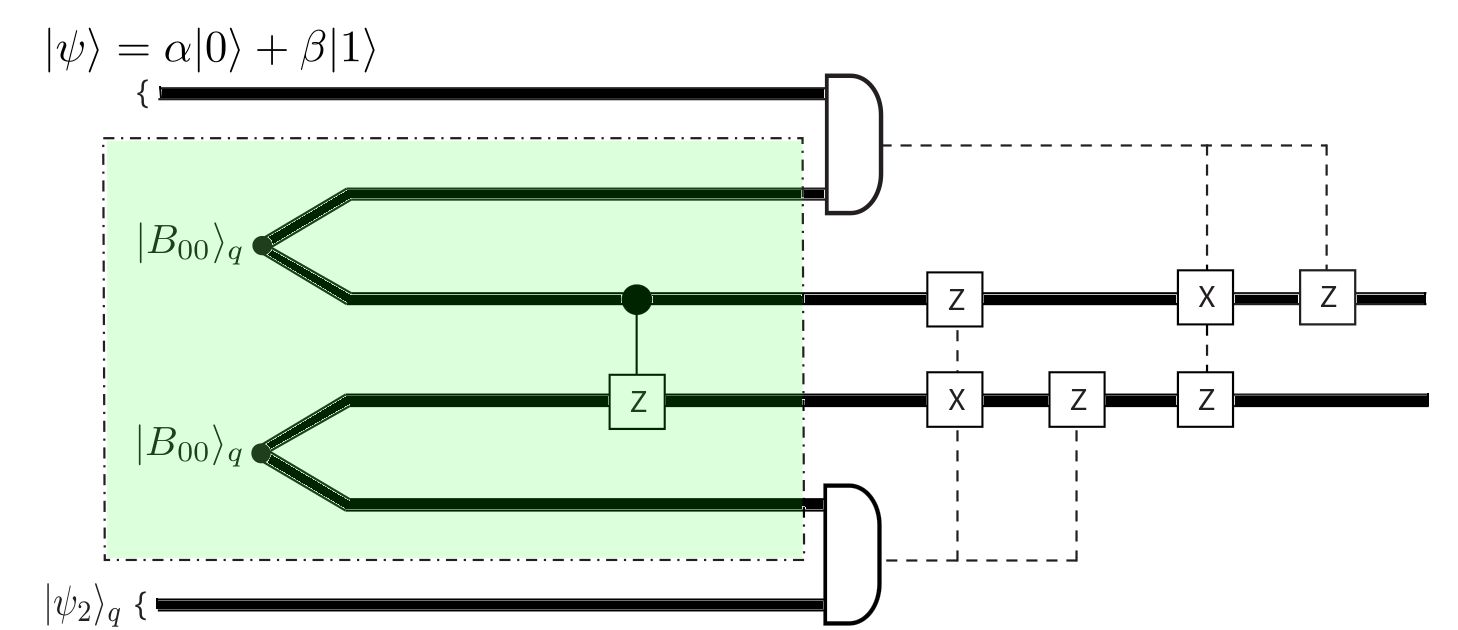
\includegraphics[scale=.20]{immagini/tele2.png}
\end{figure}
\vspace{20pt}
The entangling gate has gone into the preparation stage! This can be manifactured  off-line probabilistically \textbf{without} spoiling the quantum information when it fails.\\

\end{center}
\end{frame}

%------------------------------------------
\begin{frame}
\begin{center}

\begin{figure}[!htb]
\centering
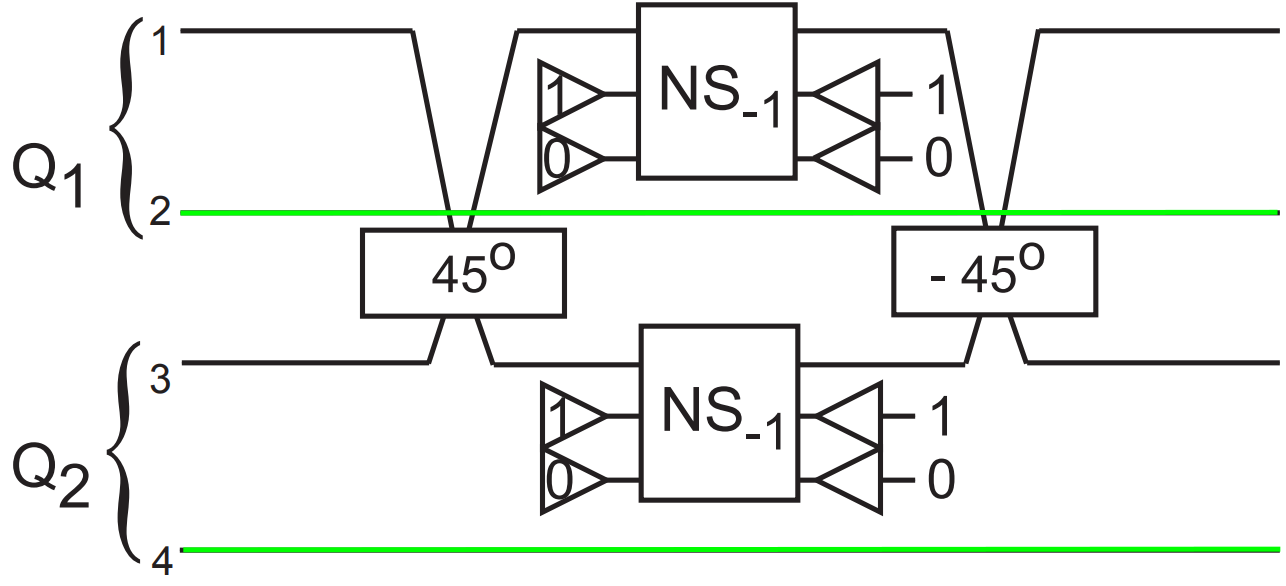
\includegraphics[scale=.25]{immagini/railColour.png}
\end{figure}
\begin{equation*}
p = \frac{1}{4} \times \frac{1}{4} = \frac{1}{16}
\end{equation*}

Remember that only modes $1$ and $3$ interact. Thus we need to teleport only two modes, not the full dual rail encoding.\\

\end{center}
\end{frame}

%------------------------------------------
\begin{frame}
\begin{center}

The Bell state $\frac{\ket{01} + \ket{10}}{\sqrt{2}}$ can be built with a $50/50$ BS:
\begin{figure}[!htb]
\centering 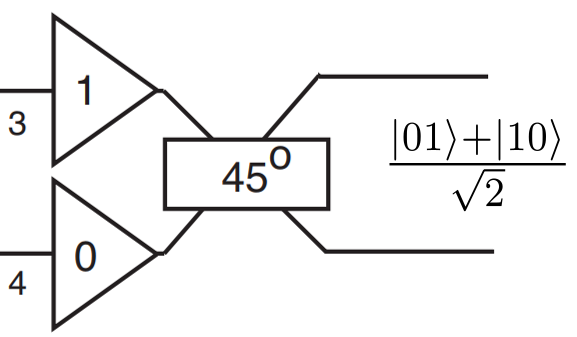
\includegraphics[scale=.20]{immagini/entaGeneration.png} 
\end{figure}

\begin{block}{}
\begin{center}
How to perform Bell measurements with linear optics?
\end{center}
\end{block}

\end{center}
\end{frame}


%------------------------------------------
\begin{frame}
\begin{center}

Teleportation of mode $1$ in mode $4$.
\begin{figure}[!htb]
\centering
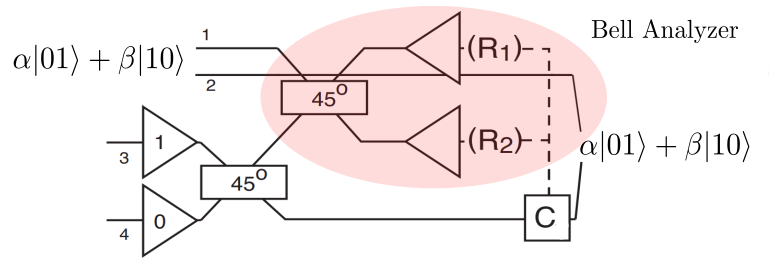
\includegraphics[scale=.4]{immagini/tele5.png}
\end{figure}
The attempted Bell measurement consist in a beamsplitter between $1$ \& $3$ and photon counting, followed by a control $C$.\\
A qubit in modes $1$ \& $2$ gets encoded in $4$ \& $2$.

\end{center}
\end{frame}

%------------------------------------------
\begin{frame}
\begin{center}

This is \textbf{probabilistic} heralded teleportation!
\begin{align*}
& R_1 = 0, R_2 = 1 \quad \frac{1}{2} \left( \alpha \ket{01} + \beta \ket{10} \right)\\
& R_1 = 1, R_2 = 0 \quad \frac{1}{2} \left( - \alpha \ket{01} + \beta \ket{10} \right) \rightarrow \text{correct}\\
\end{align*}

If a even number of photon is detected the quantum information is lost!\\	

Success probability $p = \frac{1}{2}$.

\end{center}
\end{frame}

%------------------------------------------
\begin{frame}
\begin{center}
Putting everything together:

\begin{figure}[!htb]
\centering
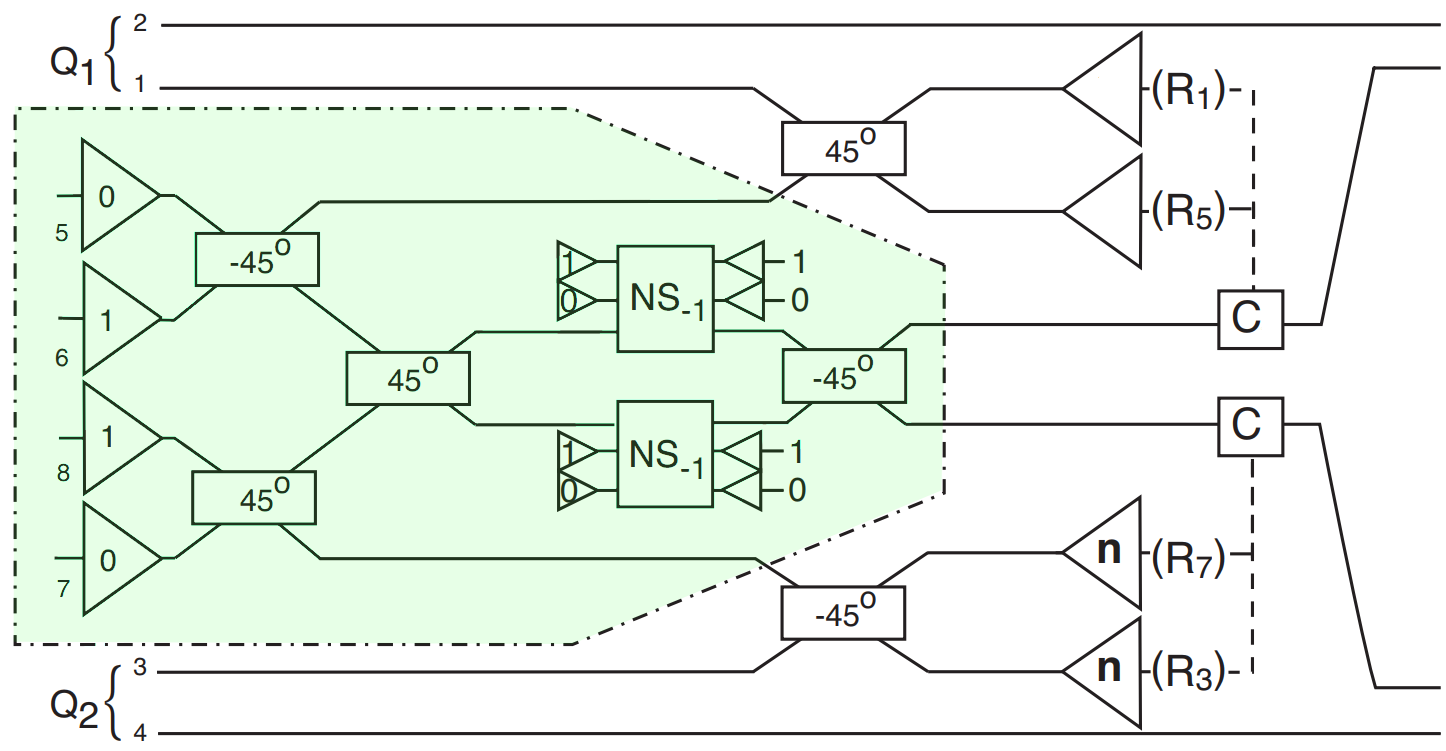
\includegraphics[scale=.20]{immagini/together.png}
\end{figure}

Success probability $ p = \frac{1}{4}$.

\end{center}
\end{frame}

%------------------------------------------
\begin{frame}{Enhanced teleportation}
\begin{center}
\begin{block}{}
\begin{center}
Deterministic Bell measurements with linear optics are impossible (Calsamiglia, 1999).
\end{center}
\end{block}
\vspace{15pt}
However the error probability $p$ for teleportation can be reduced $p \rightarrow 0$ by employing a growing entangled resource to be generated offline.\\
\vspace{10pt}
Without additional resource the previous protocol ($p = \frac{1}{2}$) is optimal.

\end{center}
\end{frame}

%------------------------------------------
\begin{frame}
\begin{center}

Offline resource on $2n$ modes:
\begin{equation*}
\ket{t_n} = \frac{1}{\sqrt{n+1}} \sum_{j = 0}^{n} \ket{1}^{j} \ket{0}^{n-j} \ket{0}^{j} \ket{1}^{n-j}
\end{equation*}

The BS is replaced by a Quantum Fourier Transform (QFT), whose action on the modes $a_j$ is:

\begin{equation*}
F^{n+1}_{kj} = \frac{e^{i \frac {2 \pi k j}{n+1}}}{\sqrt{n+1}}
\end{equation*}

Being a unitary operator it can be decomposed in a network of BS and phase shifter with $O \left( n \log n \right)$ elements for a maximum depth of $O \left( \log n \right)$.

\end{center}
\end{frame}

%------------------------------------------
\begin{frame}
\begin{center}

Count photons on the original mode and the first $n$ modes of $\ket{t_n}$. Each modes gives $r_j$ photons.

\begin{figure}[!htb]
\centering
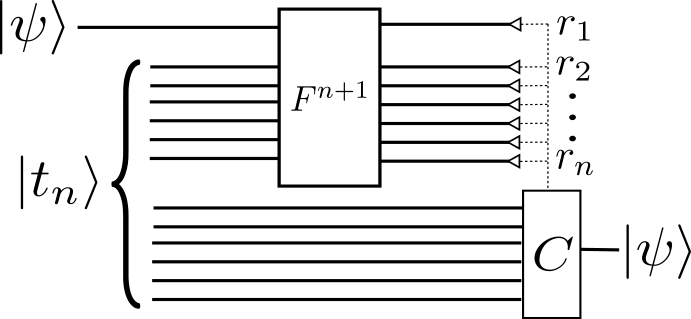
\includegraphics[scale=.60]{immagini/fourier2.png}
\end{figure}

\end{center}
\end{frame}

%------------------------------------------
\begin{frame}
\begin{center}

%TODO Valutare se aggiungere la dimostrazione (probabilmente si va troppo nel tecnico e diventa lunga
Given $k = \sum r_j$ the total number of photon detected, the input qubit is teleported in mode number $n+k$. Example (for $n = 2$):

\begin{figure}[!htb]
\centering
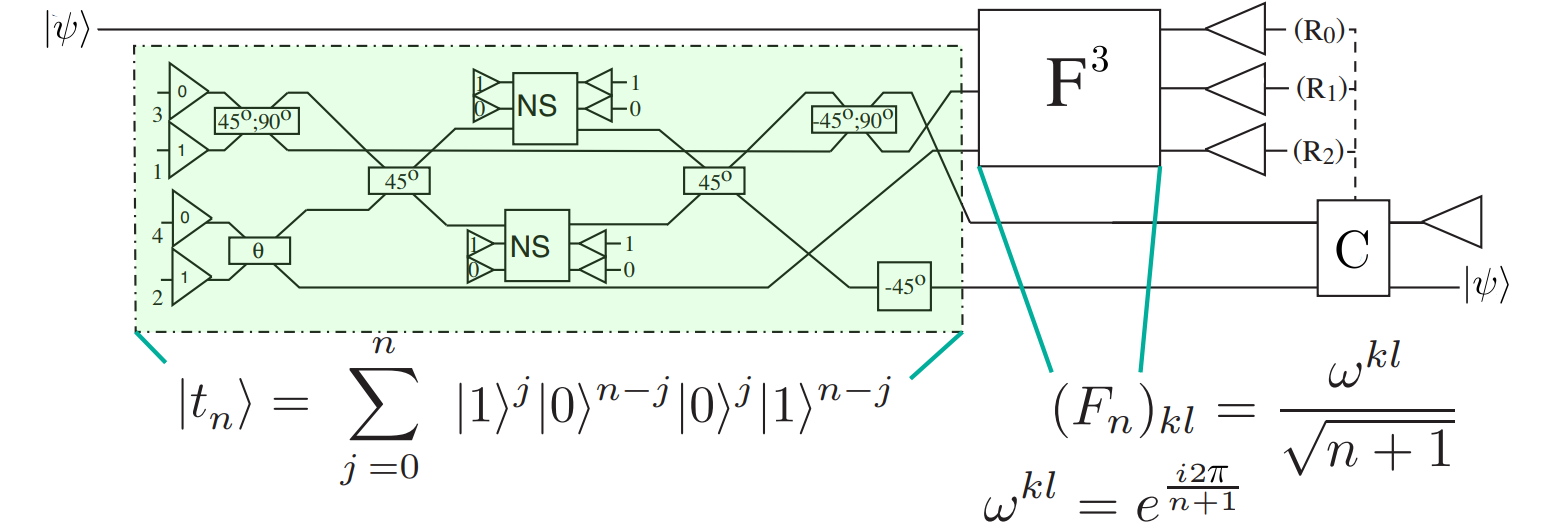
\includegraphics[scale=.20]{immagini/fourier.png}
\end{figure}

\end{center}
\end{frame}

%------------------------------------------
\begin{frame}
\begin{center}
The failure probability of teleportation is $p = \frac{1}{n+1}$.\\
\vspace{10pt}
CSIGN requires two resource states $\ket{t_n}$. The gate must be applied to every possible couple of modes, leading to:

\begin{align*}
\ket{t_n}' & = \sum_{j} \left( -1 \right)^{\left( n-j \right) \left( n-i \right)} \ket{1}^{j} \ket{0}^{n-j} \ket{0}^j \ket{1}^{n-j} \\
& \otimes \ket{1}^{i} \ket{n-i} \ket{0}^i \ket{1}^{n-i}
\end{align*}

\end{center}
\end{frame}

%------------------------------------------
\begin{frame}
\begin{center}
The failure probability for a CSIGN using $\ket{t_n}'$ is:
\begin{equation*}
p = 1-\left( \frac{n}{n+1} \right) ^2 < p_{thr}
\end{equation*}

Choose $n$ large enough that the failure probability is lower than the \textbf{threshold} for fault tolerant quantum computation.\\
\vspace{20pt}
This proves linear optics can implement \textbf{efficiently} (with polynomial overhead) a quantum computer!


\end{center}
\end{frame}


%------------------------------------------
\begin{frame}
\begin{center}

KLM showed that the required number of elementary operations needed to implement the offline resource $\ket{t_n}$ is $2^{O \left( \sqrt{n} \right)}$.
\begin{block}{}
\begin{center}
$n$ is a constant it doesn't affect the resource requirement in the scaling of the quantum computer.
\end{center}
\end{block}
For a failure probability of $p = 0.5 \%$, $n = 400$ is required, with at least $10^6$ elementary operations.\\
\vspace{10pt}
The resources for a single gate can become astronomic!

\begin{block}{}
\begin{center}
This is a proof of concept, more feasible approach to perform quantum computing with optics are needed.
\end{center}
\end{block}{}

\end{center}
\end{frame}

\begin{comment}
%------------------------------------------
\begin{frame}
\begin{center}
This is a proof of concept, more feasible approach to perform quantum computing with linear optics are needed:

\begin{itemize}
\item Improve teleportation with hybrid CV-digital techniques.
\item Error correcting codes (if a gate fails the information is not destroyed).
\item Cluster state - One way computation.
\end{itemize}

\end{center}
\end{frame}
\end{comment}

%------------------------------------------
\begin{frame}{Teleportation}
\begin{center}
The teleportation of a gaussian state is deterministic.

\begin{figure}[!htb]
\centering
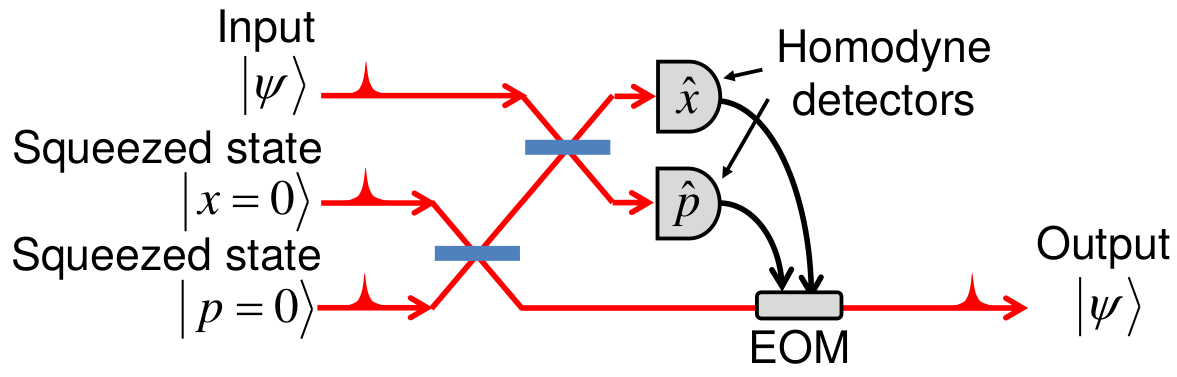
\includegraphics[scale=.25]{immagini/cv.png}
\end{figure}

%TODO Add a number for the fidelity precision in experiments.

The squeezing ratio limits the fidelity. An hybrid qubit could be:
\begin{equation*}
\ket{\psi} = c_0 \ket{01} \ket{\alpha} + c_1 \ket{10} \ket{-\alpha}
\end{equation*}

\end{center}
\end{frame}

%------------------------------------------
\begin{frame}{One way quantum computing}
\begin{center}
All the computational effort is transferred offline by producing an entangled cluster state universal for computation.

\begin{figure}[!htb]
\centering
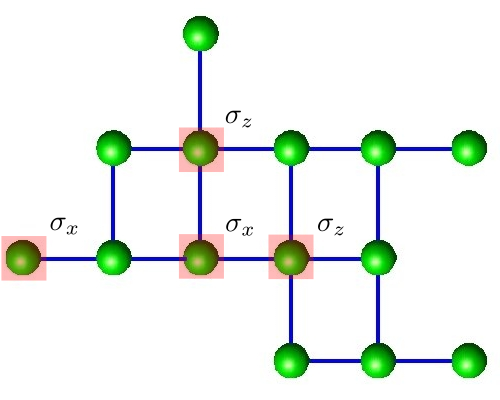
\includegraphics[scale=.4]{immagini/cluster2.png}
\end{figure}

The computation is done through single qubit measurements on the cluster.

\end{center}
\end{frame}

%------------------------------------------
\begin{frame}{Photonic architecture}
\begin{center}

\textbf{Pros}:

\begin{itemize}
\item Photons makes excellent flying qubits.
\item Negligible stochastic noise.
%\item Potentially THz frequency quantum operations.
\item Does not require mK temperatures (actually efficient detectors are superconductive).
%\item CMOS compatible, manufacturable.
\item No atomic-scale fabrication.
%\item No quantum cross-talk.
\end{itemize}

\textbf{Cons}:

\begin{itemize}
\item Photon loss (erasure channel).
\item Difficult to create entanglement.
\end{itemize}

\end{center}
\end{frame}


%------------------------------------------
\begin{frame}
\begin{center}

%Jeremy O'Brien is the CEO of PsiQuantum, a society based in Palo Alto which is pursuing integrated photonic quantum technology.

%\begin{figure}[!htb]
%\centering
%
\includegraphics[scale=.20]{immagini/psi2.jpg}
%\end{figure}

Photonic technology can be integrated using silica waveguides on a silicon chip.

\begin{figure}[!htb]
\centering
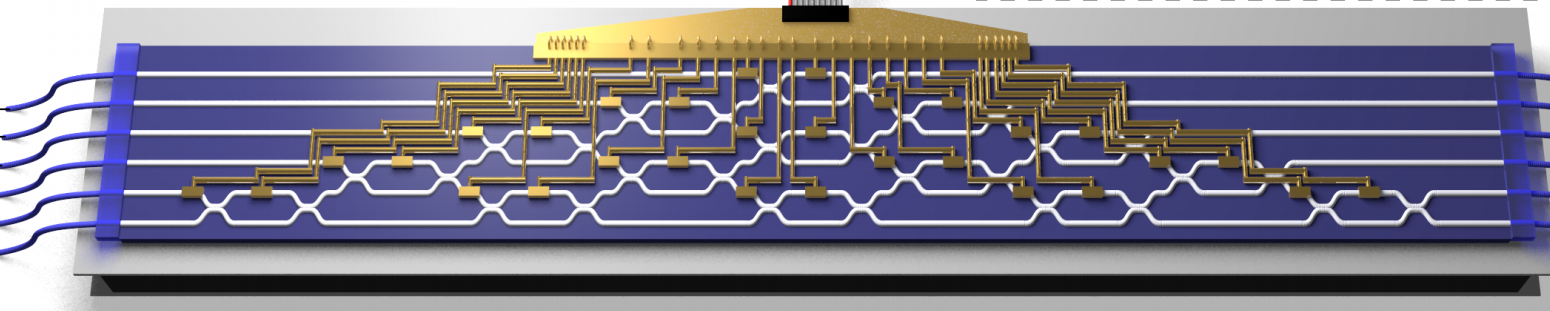
\includegraphics[scale=.20]{immagini/integrated.png}
\end{figure}

Picture taken from ``Universal Linear Optics'' (Carolan, 2015).

\end{center}
\end{frame}


%------------------------------------------
\begin{frame}{Technological problems}
\begin{center}
\begin{itemize}
\item Reliable source of single photons (above the threshold for EC)
%Not emitting a photon can be seen as an instance of photon loss (ereasure channel) to be corrected. A certain amount of photon loss can be tolerated in virtue of the threshold theorem.
\item Reliable detector (superconductors)
\item Synchronization of sources.

SPDC emits an entangled pair at random time, it is heralded but how to synchronize photon emission from different sources? 

\begin{figure}[!htb]
\centering
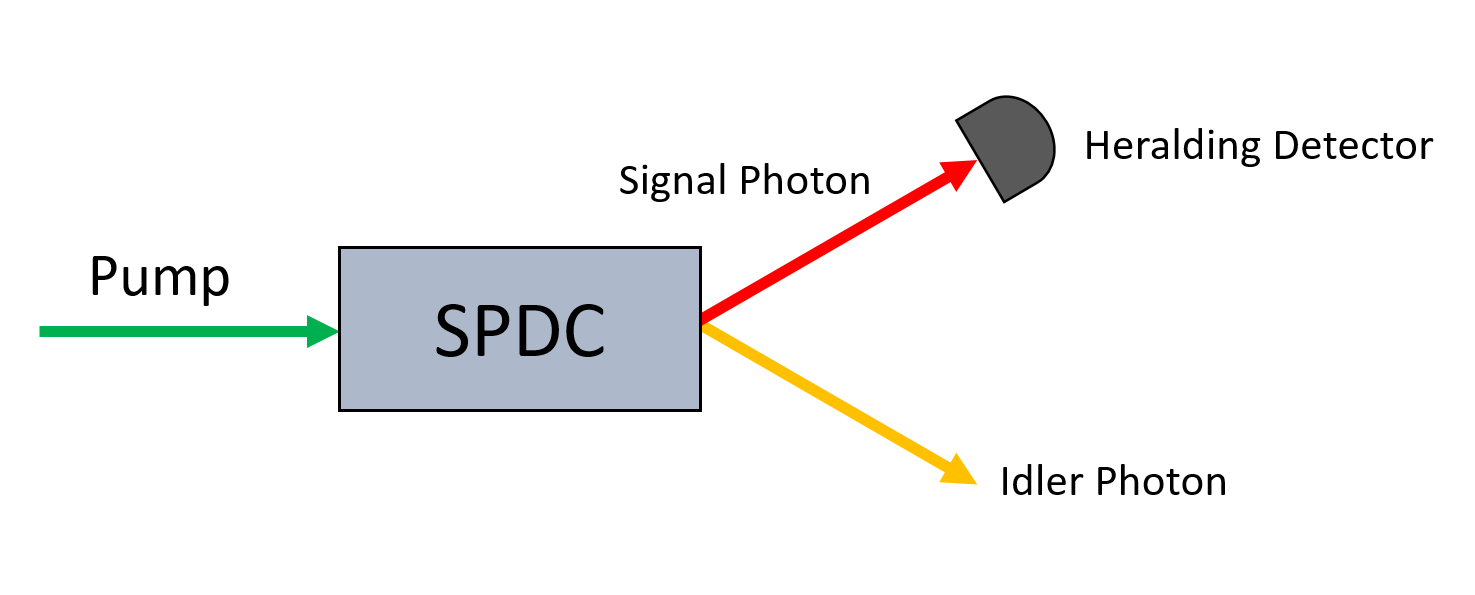
\includegraphics[scale=.20]{immagini/spdc.png}
\end{figure}

%Time multiplexing (Heuck, 2018).
Generation of a clock?
\end{itemize}

\end{center}
\end{frame}

\begin{frame}
\begin{center}
To apply the threshold theorem all the gates must be below the same level of noise. Also if they entangle qubit $1$ with qubit $N \gg 1$.\\
Entanglement between non-adjacent qubits can be done by a series of SWAP (error accumulates) or via teleportation with offline distilled entanglement.\\

\begin{figure}[!htb]
\centering
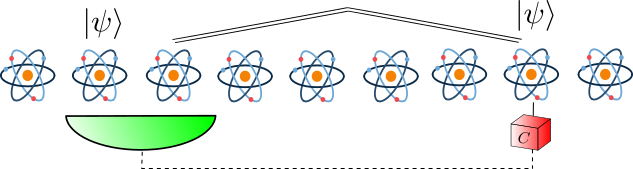
\includegraphics[scale=.50]{immagini/teleIon.png}
\end{figure}

\begin{block}{}
\begin{center}
\textbf{Connectivity problem - Qubit Bus!}
\end{center}
\end{block}

\end{center}
\end{frame}

\begin{frame}
\begin{center}
In a photonic architecture the relevant qubits can simply come closer travelling in the integrated waveguide.

\begin{figure}[!htb]
\centering
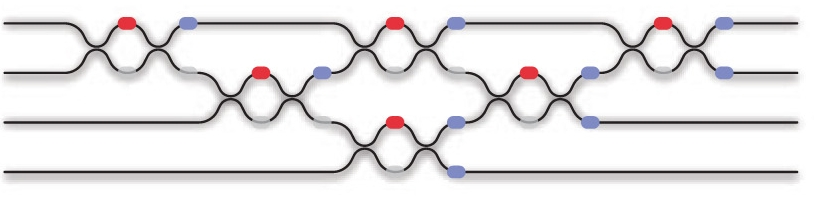
\includegraphics[scale=.40]{immagini/come.jpg}
\end{figure}

\end{center}
\end{frame}

\begin{frame}
\begin{center}
Integrated photonic circuits will have limited programmability (with respect to current platform).\\

They might come in printed modules: QFT, QPE, Grover, ...\\

High level quantum programming will consist in putting together modules via demultiplexing:

\begin{figure}[!htb]
\centering
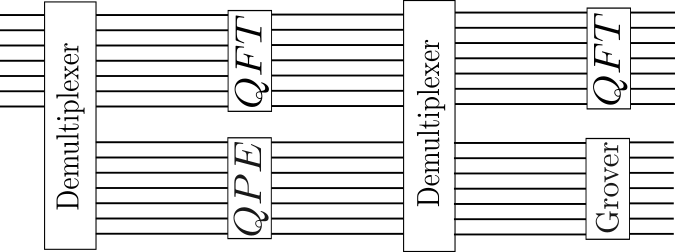
\includegraphics[scale=.50]{immagini/modular.png}
\end{figure}

\end{center}
\end{frame}

%------------------------------------------
\begin{frame}
\begin{center}

\begin{quote}
``There are a million ways to make one qubit...\\
...But only one way to make a million qubits''\\
\hfill (Terry Rudolph)
\end{quote}
\vspace{20pt}
\Huge{Thanks!}

\end{center}
\end{frame}

%------------------------------------------
\begin{frame}
\begin{center}

\begin{block}{}
\begin{center}
What if we don't have feedforward measurements? 
\end{center}
\end{block}

\begin{figure}[!htb]
\centering
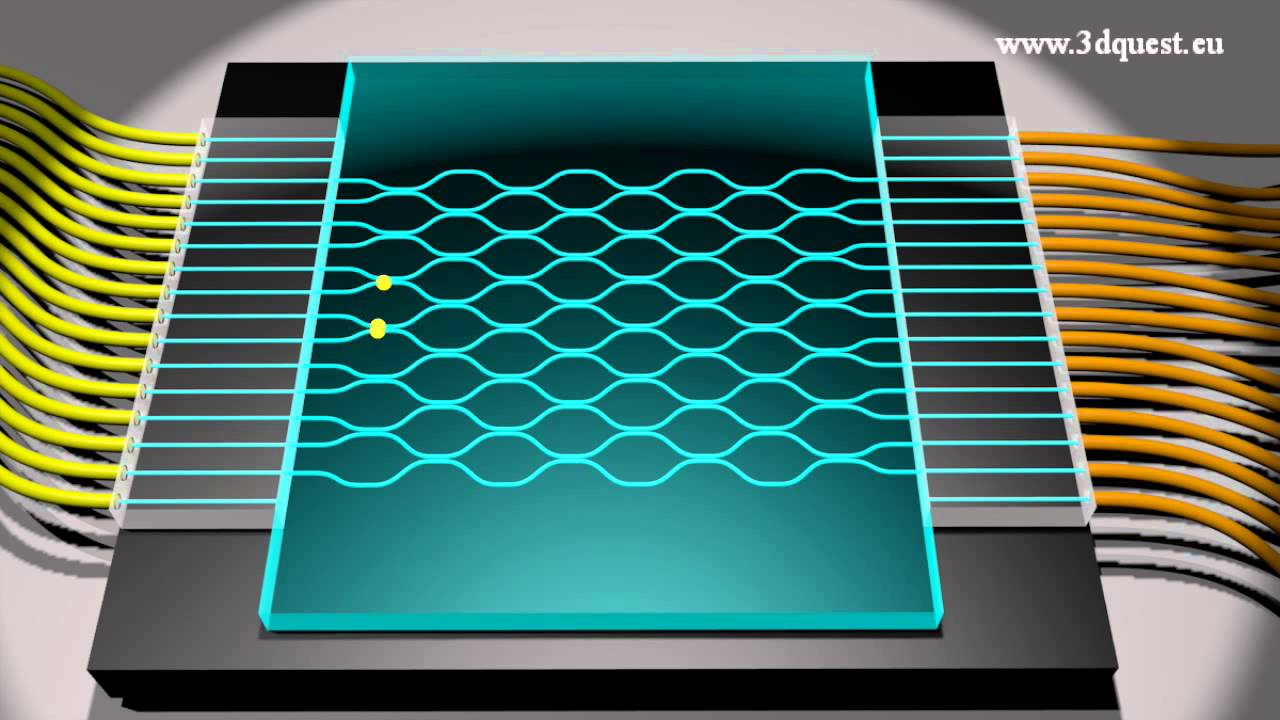
\includegraphics[scale=.20]{immagini/Bosonsampling3.jpg}
\end{figure}

The model is called BosonSampling and is still hard to simulate classically (Aaronson, Arkhipov 2013).

\end{center}
\end{frame}



%------------------------------------------
\begin{frame}
\begin{center}

\begin{figure}[!htb]
\centering
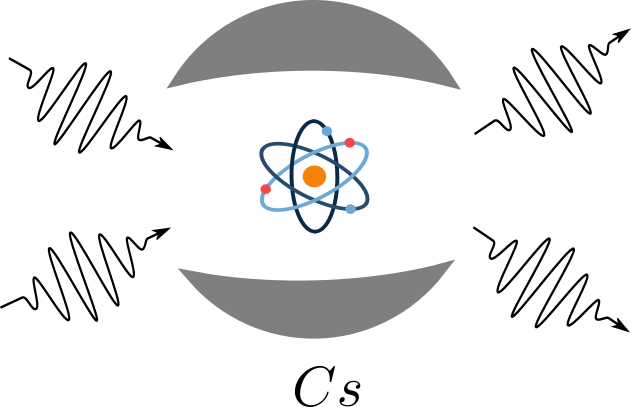
\includegraphics[scale=.50]{immagini/cavityQED.png}
\end{figure}
\vspace{15pt}

Non linear effects in QED cavities (Turchette, 1995).

\end{center}
\end{frame}

\begin{frame}
\begin{center}
Right or left circular polarization codify the qubit:
\begin{align*}
& \ket{1^{-} 1^{-}} \rightarrow \ket{1^{-} 1^{-}} \\
& \ket{1^{+} 1^{-}} \rightarrow e^{i \phi_a} \ket{1^{+} 1^{-}} \\
& \ket{1^{-} 1^{+}} \rightarrow e^{i \phi_b} \ket{1^{+} 1^{-}} \\
& \ket{1^{+} 1^{+}} \rightarrow e^{i \left( \phi_a +\phi_b + \Delta \right)} \ket{1^{+} 1^{+}}
\end{align*}

\begin{align*}
\phi_{a} &= \left( 17.5 \pm 1 \right) \degree\\
\phi_{b} &= \left( 12.5 \pm 1 \right) \degree\\
\Delta &= \left( 16 \pm 3 \right) \degree
\end{align*}

\end{center}
\end{frame}

%------------------------------------------
\begin{frame}
\begin{center}

Mixing two modes in a \textbf{two} photon absorption material, with low single photon absorption and low loss.

\begin{figure}[!htb]
\centering
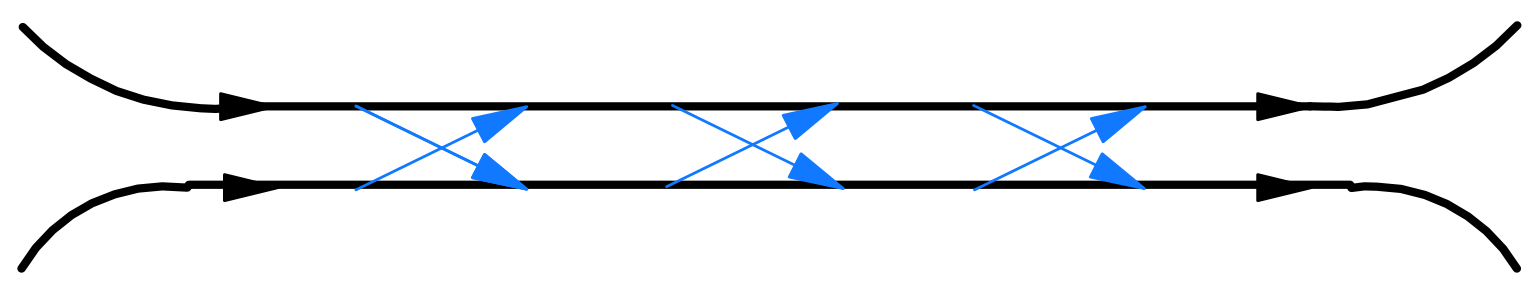
\includegraphics[scale=.20]{immagini/zeno.png}
\end{figure}

Effectively suppress HOM via Zeno effect and performs $\sqrt{SWAP}$ (Franson, 2004).\\


\end{center}
\end{frame}


\end{document}